\documentclass[12pt]{article}
\usepackage{amsmath}
\usepackage{amssymb}
\usepackage[letterpaper,top=0.85in,bottom=1in,left=0.75in,right=0.75in,centering]{geometry}
%\usepackage{fancyhdr}
\usepackage{enumerate}
%\usepackage{lastpage}
\usepackage{multicol}
\usepackage{graphicx}

\reversemarginpar

%\pagestyle{fancy}
%\cfoot{}
%\lhead{Math 1560}\chead{Test \# 1}\rhead{May 18th, 2017}
%\rfoot{Total: 10 points}
%\chead{{\bf Name:}}
\newcommand{\points}[1]{\marginpar{\hspace{24pt}[#1]}}
\newcommand{\skipline}{\vspace{12pt}}
%\renewcommand{\headrulewidth}{0in}
\headheight 30pt

\newcommand{\di}{\displaystyle}
\newcommand{\abs}[1]{\lvert #1\rvert}
\newcommand{\len}[1]{\lVert #1\rVert}
\renewcommand{\i}{\mathbf{i}}
\renewcommand{\j}{\mathbf{j}}
\renewcommand{\k}{\mathbf{k}}
\newcommand{\R}{\mathbb{R}}
\newcommand{\aaa}{\mathbf{a}}
\newcommand{\bbb}{\mathbf{b}}
\newcommand{\ccc}{\mathbf{c}}
\newcommand{\dotp}{\boldsymbol{\cdot}}
\newcommand{\bbm}{\begin{bmatrix}}
\newcommand{\ebm}{\end{bmatrix}}       
\DeclareMathOperator{\proj}{proj}            
                  
\begin{document}


\author{Instructor: Sean Fitzpatrick}
\thispagestyle{empty}
\vglue1cm
\begin{center}
{\bf MATH 1410 - Tutorial \#3 Solutions}
\end{center}


Additional practice: (\textbf{do not submit}).
\begin{enumerate}
\item Given $\vec{v}=\langle 3,-4,1\rangle$ and $\vec{w} = \langle -2,1,5\rangle$, compute:
\begin{enumerate}
\item $4\vec{v}-3\vec{w} = \langle 12, -16, 4\rangle+\langle 6, -3, -15\rangle = \langle 18, -19, -11\rangle$
\item The vector $\vec{x}$ such that $-3\vec{v}+5\vec{x}=2\vec{w}$

Adding $3\vec{v}$ to both sides, $5\vec{x}=3\vec{v}+2\vec{w}$, so
\[
\vec{x}=\frac35\vec{v}+\frac25\vec{w}=\langle \frac95, -\frac{12}{5}, \frac35\rangle+\langle -\frac45,\frac25, 2\rangle = \langle 1, -2, \frac{13}{5}\rangle.
\]
\item $\vec{v}\dotp (3\vec{w})$, $(3\vec{v})\dotp \vec{w}$, and $3(\vec{v}\dotp \vec{w})$

All three are equal to
\[
3(3(-2)-4(1)+1(5))=3(-5)=-15.
\]
\item $\proj_{\vec{v}}\vec{w}$ and $\proj_{\vec{w}}\vec{v}$
\[
\proj_{\vec{v}}\vec{w} = \left(\frac{\vec{v}\dotp\vec{w}}{\vec{v}\dotp\vec{v}}\right)\vec{v}=-\frac{5}{26}\langle 3,-4,1\rangle.
\]
\[
\proj_{\vec{w}}\vec{v} = \left(\frac{\vec{w}\dotp\vec{v}}{\vec{w}\dotp\vec{w}}\right)\vec{w} = -\frac{5}{30}\langle -2,1,5\rangle.
\]
\item Vectors $\vec{w}_{\parallel}$ and $\vec{w}_{\bot}$ such that $\vec{w}_{\parallel}$ is parallel to $\vec{v}$, $\vec{w}_{\bot}$ is orthogonal to $\vec{v}$, and $\vec{w}_{\parallel}+\vec{w}_{\bot}=\vec{w}$.

The vector $\vec{w}_\parallel$ is given by $\vec{w}_\parallel = \proj_{\vec{v}}\vec{w} = -\frac{5}{26}\langle 3,-4,1\rangle$.

The vector $\vec{w}_\bot$ is given by
\[
\vec{w}_\bot = \vec{w}-\vec{w}_\parallel = \langle -2,1,5\rangle -\left\langle \frac{-15}{26},\frac{20}{26},-\frac{5}{26}\right\rangle = \left\langle -\frac{37}{26}, \frac{6}{26}, \frac{135}{26}\right\rangle.
\]
\end{enumerate}
\end{enumerate}

\newpage
%\thispagestyle{empty}
\textbf{Assigned problems}:
  \begin{enumerate}
    \item Let $\vec{v} = \langle 4,3\rangle$ and $\vec{w} = \langle 2,3\rangle$.
    \begin{multicols}{2}
    \begin{enumerate}
    \item Compute $\proj_{\vec{v}}\vec{w}$ and $\proj_{\vec{w}}\vec{v}$.
    
    \begin{align*}
    \proj_{\vec{v}}\vec{w}& = \left(\frac{\vec{v}\dotp\vec{w}}{\vec{v}\dotp\vec{v}}\right)\vec{v}\\
    & = \frac{8+9}{16+9}\langle 4,3\rangle\\
    & = \frac{17}{25}\langle 4,3\rangle = \left\langle \frac{68}{25},\frac{51}{25}\right\rangle
    \end{align*}
    and
    \begin{align*}
    \proj_{\vec{w}}\vec{v}&=\left(\frac{\vec{w}\dotp\vec{v}}{\vec{w}\dotp\vec{w}}\right)\vec{w}\\
    & = \frac{9+8}{4+9}\langle 2,3\rangle\\
    &=\frac{17}{13}\langle 2,3\rangle = \left\langle \frac{34}{13},\frac{51}{13}\right\rangle.
    \end{align*}
    \columnbreak
    \item Sketch $\vec{v}$, $\vec{w}$, $\proj_{\vec{v}}\vec{w}$, and $\proj_{\vec{w}}\vec{v}$ on one set of coordinate axes.
    \begin{center}
    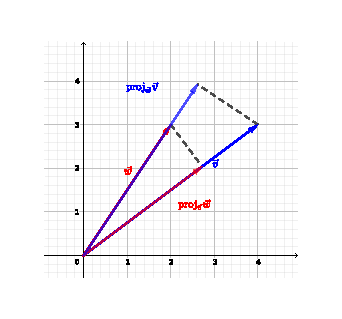
\includegraphics[width=\columnwidth]{T3-1}
    \end{center}
    \end{enumerate}
    \end{multicols}
   
    
    \item Show that for \textbf{any} vectors $\vec{u}$, $\vec{v}$, and $\vec{w}$ in $\R^2$,
    \[
    \vec{u}\dotp (\vec{v}+\vec{w}) = \vec{u}\dotp\vec{v}+\vec{u}\dotp \vec{w}.
    \]
    Then, illustrate the result with an example.
    
    \bigskip
    
    Let $\vec{u}=\langle u_1,u_2\rangle$, $\vec{v}=\langle v_1,v_2\rangle$, and $\vec{w}=\langle w_1,w_2\rangle$ for some real numbers $u_1,u_2,v_1,v_2,w_1,w_2$. Then
    \begin{align*}
    \vec{u}\dotp (\vec{v}+\vec{w}) & = \langle u_1,u_2\rangle\dotp(\langle v_1,v_2\rangle +\langle w_1,w_2\rangle)\tag{subsituting expressions}\\
    & = \langle u_1,u_2\rangle\dotp\langle v_1+w_1,v_2+w_2\rangle\tag{definition of vector addition}\\
    & = u_1(v_1+w_1)+u_2(v_2+w_2)\tag{definition of dot product}\\
    & = (u_1v_1+u_1w_1)+(u_2v_2+u_2w_2) \tag{distributive property of $\R$}\\
    & = (u_1v_1+u_2v_2)+(u_1w_1+u_2w_2) \tag{changing order of addition}\\
    & = \vec{u}\dotp\vec{v}+\vec{u}\dotp\vec{w} \tag{definition of dot product},
    \end{align*}
    as required.

\medskip
    
    For example, if $\vec{u}=\langle 1,2\rangle$, $\vec{v}=\langle 3,-1\rangle$, and $\vec{w} = \langle -2,4\rangle$, then
    \[
    \vec{u}\dotp(\vec{v}+\vec{w}) = \langle 1,2\rangle\dotp (\langle 3,-1\rangle +\langle -2,4\rangle)=\langle 1,2\rangle\dotp \langle 1,3\rangle = 1+6=7,
    \]
    while
    \[
    \vec{u}\dotp\vec{v}+\vec{u}\dotp\vec{w} = \langle 1,2\rangle\dotp\langle 3,-1\rangle + \langle 1,2\rangle\dotp\langle -2,4\rangle = (3-2)+(-2+8) = 7,
    \]
    so the two sides agree, as they must.
    
   
\end{enumerate}
  
\end{document}